\chapter{Introduction}\label{ch:intro}

\begin{figure}[t]
\centering
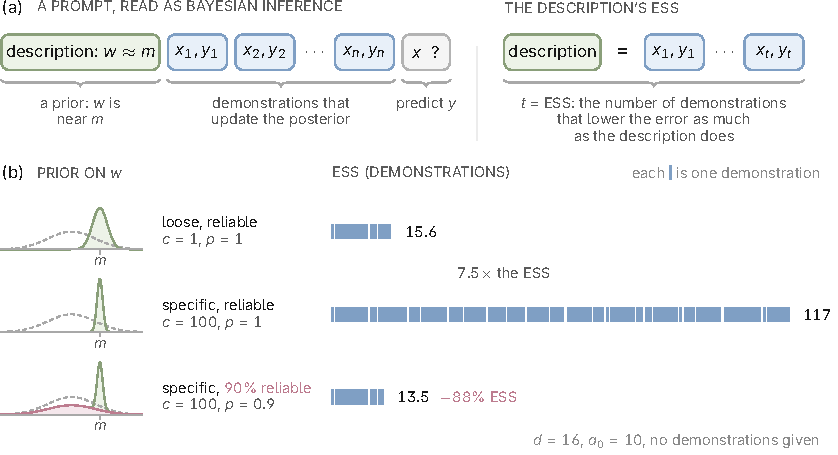
\includegraphics[width=\textwidth]{overview_sq.pdf}
\caption[Measuring a task description in demonstrations]{\textbf{Measuring a task description in demonstrations.} (a) A description provides information about a latent task $w$, and demonstrations supply additional evidence. Its predictive effective sample size (ESS) is the number of additional demonstrations a learner without the description needs to match the error it reaches with the description. The schematic on the right illustrates $n=0$. (b) Description-conditioned task distributions and their Bayes-optimal ESS at $n=0$, $d=16$, and $a_0=10$. Specificity is set by the precision $c$ of the relevant component; reliability $p$ is that component's prior probability. Pink denotes the irrelevant component. Increasing specificity greatly increases ESS when $p=1$, whereas a $10\%$ probability of irrelevance sharply limits this benefit.}
\label{fig:overview}
\end{figure}

Large language models (LLMs) are capable of in-context learning (ICL): given a prompt that specifies a task through a natural-language description, demonstrations, or both, they can predict the output for a new query input \citep{brown2020}. In practice, prompts consist mostly of system instructions, user instructions, skill files, and earlier conversation turns, which typically describe the task rather than demonstrate it \citep{mao2025,patsakis2026}. The balance shifts further as LLMs carry out increasingly long-horizon tasks \citep{kwa2025}, for which demonstrations are costly to provide.

Theories of ICL, however, have mostly focused on prompts consisting of demonstrations alone \citep{xie2022,garg2022,akyurek2023}. The few that include descriptions study only specific types, such as a descriptor that describes the input distribution \citep{huangge2025}, a set of candidate hypotheses \citep{lin2025}, or related datasets supplied as context \citep{zhu2026}; none offers a systematic treatment of descriptions. We therefore ask: how can we characterize natural-language descriptions in general to formally understand and analyze them? And how do descriptions compare, combine, and interact with demonstrations?

We study both questions through the Bayesian view of ICL, in which a model infers a latent task from the demonstrations \citep{xie2022}; a description can then be modeled as a prior over tasks. Descriptions differ in how far they narrow down the task and in whether they apply: ``write this report as an accountant'' leaves most of it open, a step-by-step workflow for each part leaves little, and either may be meant for another task. We formalize these two properties in $d$-dimensional Gaussian linear regression, a standard controlled setting for ICL \citep{garg2022,panwar2024}. Without a description, the coefficients follow a Gaussian baseline prior with variance $a_0$; a description supplies further information about them before demonstrations are observed. A mixture model separates uncertainty about where the task lies from uncertainty about whether the description applies: with probability $p$, the description is relevant, and the coefficients are Gaussian around its center with precision $c$; otherwise, it is independent of the task. We thus characterize a description by two quantities: its \emph{specificity}, set by $c$, and its \emph{reliability}, the prior probability $p$ that it is relevant (Figure~\ref{fig:overview}).

To compare descriptions with demonstrations, we adapt sample-size measures of prior impact and predictive performance \citep{wiesenfarth2020,reimherr2021,lescao2021,selby2025}. For a given learner and prediction loss, a description's \emph{predictive effective sample size} (ESS) at $n$ demonstrations is the additional number of demonstrations needed without the description to reach the same expected error. Standard prior ESS instead matches information, which requires an explicit prior \citep{morita2008}; a network or a language model also brings prior knowledge, acquired in training, but holds it only implicitly in its weights, so only its error can be compared. Computing ESS for both the Bayes-optimal predictor and trained models distinguishes the information available under the statistical model from the benefit realized by a learner.

We then ask how closely trained learners attain the Bayes-optimal ESS. Transformers trained from scratch on the Gaussian model receive each description as an input token and must learn its precision and reliability from their training data. Pretrained language models cannot learn these from the task distribution, so the prompt must state them, as probabilistic statements in numerical mean-estimation tasks. Using a stated precision requires weighting the description and the demonstrations by their precisions, a computation that reasoning may help a model carry out, so we compare models with reasoning enabled and disabled.

% An in-context learner can learn about a task in two ways: a prompt can describe what to do, or it can demonstrate the desired behavior. Most practical prompts combine the two \citep{brown2020}, and task descriptions also appear in system instructions and the files used to configure coding agents \citep{chatlatanagulchai2025}. Yet we lack a common scale for comparing the information supplied by a description with that supplied by examples. When should a precise description replace many demonstrations? When can examples help a learner recognize that a description does not apply?

\section{Main Findings}

Our main findings are as follows:
\begin{itemize}[leftmargin=*,itemsep=2pt,topsep=3pt]
\item \textbf{Precision and dimension determine the value of reliable descriptions.} With fixed positive integer precision $c$, zero-demonstration ESS approaches $c+d+1$ as the baseline prior becomes diffuse (Chapter~\ref{ch:specificity}).
\item \textbf{Uncertain relevance limits zero-demonstration ESS.} Any fixed positive probability of irrelevance imposes a finite ceiling as precision grows. For $d=16$, baseline variance $a_0=10$, and $c=100$, lowering reliability from $1$ to $0.9$ reduces ESS from approximately $117$ to $13.5$. With demonstrations, a learner can also infer whether the description is relevant (Chapter~\ref{ch:reliability}).
\item \textbf{Description use depends on training for Transformers, and on reasoning for language models.} Meta-trained Transformers approach the Bayes-optimal ESS, and their fitted description weight follows the reliability of their training data, even when test descriptions are more reliable. For most pretrained language models tested, enabling reasoning brings their use of stated precision close to the Bayesian reference. When descriptions are in fact unreliable and the prompt says so, GPT-6 Sol with reasoning also matches the reference, which requires inferring relevance from the demonstrations (Chapters~\ref{ch:networks}--\ref{ch:llm}).
\end{itemize}

\section{Outline}\label{sec:outline}

Chapter~\ref{ch:background} reviews in-context learning and its Bayesian interpretation, in-context linear regression and its squared error, the effective sample size of a prior, and robust mixture priors, together with related work. Chapter~\ref{ch:setup} presents the framework: tasks and demonstrations, descriptions as uncertain task information, prediction error, and predictive ESS. Chapter~\ref{ch:specificity} derives the value of a reliable description, with its proofs and the analysis of partial descriptions. Chapter~\ref{ch:reliability} derives the cost of unreliability, with its proofs and the analysis of the Bayesian predictor assuming relevance under misspecification. Chapter~\ref{ch:networks} tests meta-trained Transformers, with their training details and further networks. Chapter~\ref{ch:llm} tests pretrained language models on numerical prediction tasks with explicit probabilistic descriptions, with the evaluation details and further experiments on stated reliability and on a semantic classification task. Chapter~\ref{ch:conclusion} discusses the findings and their limitations, and outlines future work. Appendix~\ref{app:llm-tables} reports the language-model tables at every evaluated demonstration count.
